%%%%%%%%%%%%%%%%%%%%%%%%%%%%%%%%%%%%%%%%%
% Short Sectioned Assignment
% LaTeX Template
% Version 1.0 (5/5/12)
%
% This template has been downloaded from:
% http://www.LaTeXTemplates.com
%
% Original author:
% Frits Wenneker (http://www.howtotex.com)
%
% License:
% CC BY-NC-SA 3.0 (http://creativecommons.org/licenses/by-nc-sa/3.0/)
%
%%%%%%%%%%%%%%%%%%%%%%%%%%%%%%%%%%%%%%%%%

%----------------------------------------------------------------------------------------
%	PACKAGES AND OTHER DOCUMENT CONFIGURATIONS
%----------------------------------------------------------------------------------------

\documentclass[paper=a4, fontsize=11pt]{scrartcl} % A4 paper and 11pt font size

\usepackage[T1]{fontenc} % Use 8-bit encoding that has 256 glyphs
\usepackage[english]{babel} % English language/hyphenation
\usepackage{amsmath,amsfonts,amsthm} % Math packages
\usepackage{lipsum} % Used for inserting dummy 'Lorem ipsum' text into the template

\usepackage[pdftex]{graphicx}
\usepackage{epstopdf}
\DeclareGraphicsExtensions{.eps}

\usepackage{sectsty} % Allows customizing section commands
\allsectionsfont{\centering \normalfont\scshape} % Make all sections centered, the default font and small caps

\usepackage{fancyhdr} % Custom headers and footers
\pagestyle{fancyplain} % Makes all pages in the document conform to the custom headers and footers
\fancyhead{} % No page header - if you want one, create it in the same way as the footers below
\fancyfoot[L]{} % Empty left footer
\fancyfoot[C]{} % Empty center footer
\fancyfoot[R]{\thepage} % Page numbering for right footer
\renewcommand{\headrulewidth}{0pt} % Remove header underlines
\renewcommand{\footrulewidth}{0pt} % Remove footer underlines
\setlength{\headheight}{13.6pt} % Customize the height of the header

\renewcommand{\thesubsection}{\thesection.\alph{subsection}}

\numberwithin{equation}{section} % Number equations within sections (i.e. 1.1, 1.2, 2.1, 2.2 instead of 1, 2, 3, 4)
\numberwithin{figure}{section} % Number figures within sections (i.e. 1.1, 1.2, 2.1, 2.2 instead of 1, 2, 3, 4)
\numberwithin{table}{section} % Number tables within sections (i.e. 1.1, 1.2, 2.1, 2.2 instead of 1, 2, 3, 4)

\setlength\parindent{0pt} % Removes all indentation from paragraphs - comment this line for an assignment with lots of text

%----------------------------------------------------------------------------------------
%	TITLE SECTION
%----------------------------------------------------------------------------------------

\newcommand{\horrule}[1]{\rule{\linewidth}{#1}} % Create horizontal rule command with 1 argument of height

\title{	
\normalfont \normalsize 
%\textsc{university, school or department name} \\ [25pt] % Your university, school and/or department name(s)
\horrule{0.5pt} \\[0.4cm] % Thin top horizontal rule
\huge MAE 6254 Midterm Exam \\ % The assignment title
\horrule{2pt} \\[0.5cm] % Thick bottom horizontal rule
}

\author{Randy Schur} % Your name

\date{\normalsize March 28 2016} % Today's date or a custom date

\begin{document}

\maketitle % Print the title

%----------------------------------------------------------------------------------------
%	PROBLEM 1
%----------------------------------------------------------------------------------------

\section{Problem 1}
For the following system: 
\begin{align*} 
\dot{x_1} &= -x_1^3 + x_2 \\
\dot{x_2} &= x_1 - x_2^3				
\end{align*}
a) find three equilibria \\

Equilibria are at $x^*$ where $\dot{x}^*=0$. Therefore 
\begin{align*}
0 &= -x_1^3 + x_2 \\
0 &= x_1 - x_2^3
\end{align*}
This is true at:
\begin{align}
x_1^* = \begin{bmatrix}0 & 0\end{bmatrix}^T \\
x_2^* = \begin{bmatrix}1 & 1\end{bmatrix}^T \\
x_3^* = \begin{bmatrix}-1 & -1\end{bmatrix}^T 
\end{align}

b) Find the type of each equilibrium
\begin{align*}
x &= x^* + \delta x \\
\dot{x} &= \dot{x}^* + \delta \dot{x} = \frac{\partial f}{\partial x}\Bigr|_{x^*} \\
A &= \begin{bmatrix}
\frac{\partial f_1}{\partial x_1} & \frac{\partial f_1}{\partial x_2} \\ 
\frac{\partial f_2}{\partial x_1} & \frac{\partial f_2}{\partial x_2} \\ 
\end{bmatrix}
= \begin{bmatrix}
-3x_1^2 & 1 \\ 
1 & -3x_2^2 
\end{bmatrix}
\end{align*}
By evaluating matrix A at each equilibrium and finding it's eigenvalues, we can determine the type of equilibrium.\\
Equilibrium 1: 
\begin{align}
A &= \begin{bmatrix}
0 & 1\\ 
1 & 0  
\end{bmatrix}\\
\lambda &= -1,\ 1 \Rightarrow\ saddle\ point
\end{align} \\
Equilibrium 2: 
\begin{align}
A &= \begin{bmatrix}
-3 & 1\\ 
1 & -3  
\end{bmatrix}\\
\lambda &= -4,\ -2 \Rightarrow\ stable\ node
\end{align} \\
Equilibrium 3: 
\begin{align}
A &= \begin{bmatrix}
-3 & 1\\ 
1 & -3  
\end{bmatrix}\\
\lambda &= -4,\ -2 \Rightarrow\ stable\ node
\end{align} \\

\newpage

\section{Problem 2}
a) Find the equilibrium of the system:
The equilibrium is at $x^* = \begin{bmatrix}0 & 0\end{bmatrix}^T$. This makes 
\begin{align*}
\dot{x_1} &=(1+0)(0-0) = 0\\
\dot{x_2} &= 0(1+0) = 0
\end{align*}

b) Make the strongest possible statement about the stability of the system using the given Lyapunov equation:
\begin{equation}
V(x_1, x_2) = \frac{x_1^2}{1+x_1^2}+\frac{x_2^2}{1+x_2^2}
\end{equation}
$V$ is positive definite becauase $V=0$ only if $x^= \begin{bmatrix}0 & 0\end{bmatrix}^T$.
\begin{align}
\dot{V} &= \frac{\partial V}{\partial x_1}\dot{x_1} + \frac{\partial V}{\partial x_2}\dot{x_2} \\
&= \frac{(1+x_1^2)2x_1 - x_1^2(2x_1}{(1+x_1^2)^2}(1+x_1^2)^2(-x_1-x_2) + \frac{(1+x_2^2)2x_2 - x_2^2(2x_2}{(1+x_2^2)^2}x_1(1+x_1^2)^2 \\
&= (2x_1+2x_1^3 - 2x_1^3)(-x_1-x_2) + (2x_2+2x_2^3-2x_2^3)x_1\\
&= -2x_1^2
\end{align}
Therefore $\dot{V}$ is negative semi-definite, and the equilibrium is stable. We can use LaSalle's theorem to show that the equilibrium of this time-invariant system is asymptotically stable.

Let $S=\{x \in D | x_1=0 \}$. Let $x_1, x_2$ be solutions staying in $S$. $V=\dot{V}=0$ implies that $x_1=0$, and therefore $\dot{x_1}=0$. This leaves the equation for $V$ as:
\begin{equation}
0 = \frac{x_2^2}{1+x_2^2}
\end{equation}
The only solution for which this is true is $x_2=0$. By LaSalle's theorem, the equilibrium is asymptotically stable. 

The above is true for $x \in D = \mathbb{R}^2$, and additionally V is radially unbounded. Therefore, the equilibrium is globally asymptotically stable.
\newpage

\section{Problem 3}
a) Show that the given Lyapunov equation is positive definite (p.d.).
\begin{align}
V(x_1, x_2) &= \frac{3}{2} x_1^2-x_1x_2+x_2^2 \\
&= \begin{bmatrix}x_1 & x_2\end{bmatrix} \mathbf{P} \begin{bmatrix}x_1 & x_2\end{bmatrix}^T \\
&= \begin{bmatrix}x_1 & x_2\end{bmatrix} \begin{bmatrix}3/2 & -2\\ 1 & 1\end{bmatrix} \begin{bmatrix}x_1 & x_2\end{bmatrix}^T
\end{align}
$V$ is p.d. if $\mathbf{P}$ is p.d. Matrix $\mathbf{P}$ is p.d. if the eigenvalues of $[\mathbf{P}+\mathbf{P}^T]/2>0$, or equivalently if the determinant of each leading principle minor is positive.
\begin{equation}
[P+P^T]/2 = Q = \begin{bmatrix}3/2 & -\frac{1}{2}\\ -\frac{1}{2} & 1\end{bmatrix}
\end{equation}
Both leading principle minors of $\mathbf{Q}$ are positive, and therefore $V$ is positive definite. \\

b) Show that the equilibrium is asymptotically stable:
\begin{align}
\dot{V} &= \frac{\partial V}{\partial x_1}\dot{x_1} + \frac{\partial V}{\partial x_2}\dot{x_2} \\
&= (3x_1-x_2)(-x_2) + (2x_2-x_1)((x_1^2-1)x_2+x_1) \\
&= -x_1^2-x_2^2 + 2x_1^2x_2^2-x_1^3x_2 \\
&= -x_1^2(1+x_1x_2) - x_2^2(1-2x_1^2)
\end{align}
In the domain $D=\{x_1, x_2 \in \mathbb{R}\ |\ 1+x_1x_2>0,\ x_1^2<\frac{1}{2}\}$, $\dot{V}$ is negative definite, and therefore the equilibrium is asymptotically stable. \\

c) For a constant $c$, the sublevel set $\Omega_c$ of $V$ is described by an ellipse. This ellipse can be found from the equation of $V$. The equation of an ellipse is given by 
\begin{equation}
0=Ax^2+Bxy+Cy^2+Dx+Ey+F
\end{equation}
where the coefficients are calculated as functions of the semi-major ($a$) and semi-minor ($b$) axes, and angle ($\theta$) of the semi-major axis. In this case
\begin{align}
A &= \frac{3}{2} &= a^2sin^2\theta + b^2cos^2\theta \\
B &= -1 &= 2(b^2-a^2)sin\theta cos\theta \\
C &= 1 &= a^2cos^2\theta + b^2sin^2\theta \\
F &= c &= -a^2b^2
\end{align}
This system of equations can be solved for $a, b, \theta$. For a constant $c$:
\begin{align}
a^2 &= \frac{-c}{b^2} \\
b^2 &= \frac{-\frac{3}{2} \pm \sqrt{\frac{9}{4}+4cos^2\theta sin^2\theta}}{2cos^2\theta} \\
sin(2\theta) &= \frac{-1}{b(\theta)^2 + \frac{c}{b(\theta)}} 
\end{align}
Once this system of equations is solved, the semi-major axis is given by $a$, the semi-minor axis is given by $b$, the angle of the semi-major axis is given by $\theta$, and the angle of the semi-minor axis is given by $\theta+\frac{\pi}{2}$.
The ellipse described above can be seen in the contour plot of $V$.
\begin{figure}[h!]
\label{contour1}
\centering
\includegraphics[scale=0.75]{prob3_ellipse}
\caption{Contour plot of $V$. The sublevel set of $V$ is anything inside a given contour corresponding to the constant $c$.}
\end{figure} 

(d) The region of attraction (ROA) for $V$ is bounded by trajectories. This region is described by the largest sublevel set in which ${V}$ always remains. A conservative estimate of this region of attraction is given by the ellipse found when $a=4, b=1/4, \theta=0$. This region can be expanded out to the trajectories given as the limits of the domain $D$. A larger estimate of the ROA is given by the largest subset of $V$ for which $\dot{V}$ remains negative. This is true for the ellipse at $\theta=1.02, a = 5/3, b= 1$. This ellipse is shown in the image below.

\begin{figure}[h]
\label{contour2}
\centering
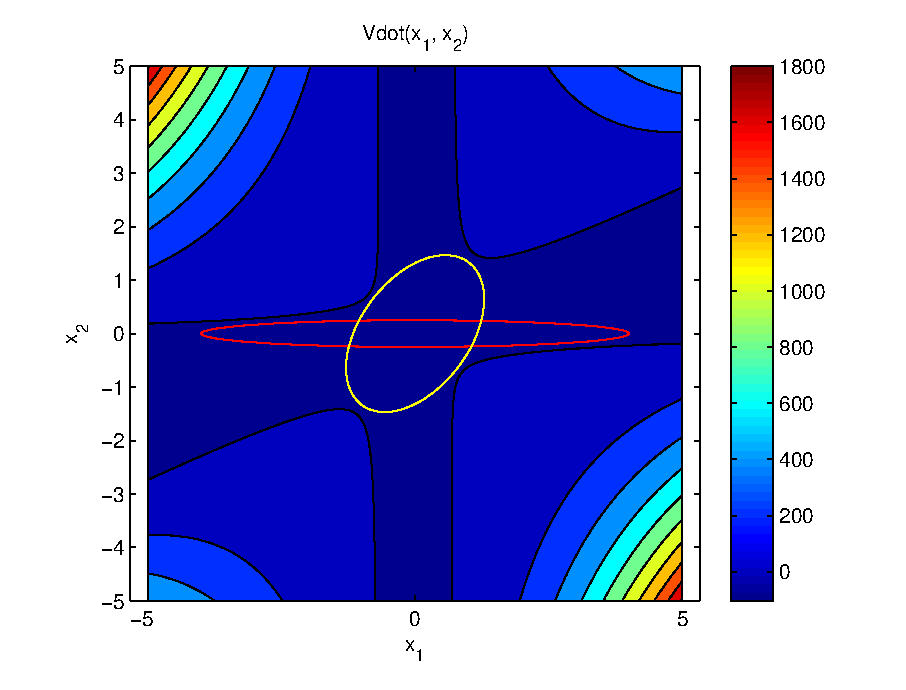
\includegraphics[scale=0.75]{prob3_ROA}
\caption{Estimates of the region of attraction plotted over a contour plot of $\dot{V}$}
\end{figure} 

\newpage

\section{Problem 4}
a) Show that $V$ is positive definite and decrescent for the given time-varying system:
\begin{align}
V(t, x_1, x_2) &= \frac{1}{2}(x_1+x_2)^2+\frac{1}{2}(1+b(t))x_1^2 \\
&\geq \begin{bmatrix}x_1 & x_2\end{bmatrix} \begin{bmatrix}2 & \frac{1}{2}\\ \frac{1}{2} & \frac{1}{2}\end{bmatrix} \begin{bmatrix}x_1 & x_2\end{bmatrix}^T = W_1(x)
\end{align}
Since $W_1(x)$ is p.d., and $V \geq W_1(x) \forall t$, $V$ must be p.d. Also, 
\begin{align}
 V(t, x_1, x_2) &= \frac{1}{2}(x_1+x_2)^2+\frac{1}{2}(1+b(t))x_1^2 \\
&\leq \begin{bmatrix}x_1 & x_2\end{bmatrix} \begin{bmatrix}3 & \frac{1}{2}\\ \frac{1}{2} & 1\end{bmatrix} \begin{bmatrix}x_1 & x_2\end{bmatrix}^T = W_2(x)
\end{align}
Since $W_2(x)$ is p.d. and $V \leq W_2(x) \forall t$, $V$ must be decrescent. \\

b) Show that the origin is globally asymptotically stable, and find the constants of the exponential bound:

First, we have already found that V is positive definite and decrescent. Additionally, because $V\rightarrow \infty \Rightarrow x \rightarrow \infty$, $V$ is radially unbounded. These properties hold for $D = \mathbb{R}^2$.
\begin{align}
\dot{V} &= \frac{\partial V}{\partial x_1}\dot{x_1} + \frac{\partial V}{\partial x_2}\dot{x_2} \\
&= (4x_1 + x_2)\dot{x_1} + (x_1+x_2)\dot{x_2} \\
&= -2x_1^2 + (2-b(t))x_1x_2 - (b(t)-1)x_2^2 \\
&\leq -2x_1^2 -2x_1x_2 - 3x_2^2 \\
&\leq -3 \lvert\lvert x \rvert\rvert
\end{align}
Therefore, V is negative definite. This holds for $D = \mathbb{R}^2$, so the equilibrium is globally exponentially stable and bounded by $\lvert\lvert x \rvert\rvert \leq 3\lvert\lvert x_0\rvert\rvert exp[-(t-t_0)]$. The constants for the exponential bound are found by
\begin{align}
W_1(x) &=\frac{1}{2}\lvert\lvert x \rvert\rvert \\
W_2(x) &=\frac{3}{2}\lvert\lvert x \rvert\rvert \\
W_3(x) &=-3\lvert\lvert x \rvert\rvert \\
k &= \frac{k_2}{k_1} = 3 \\
\gamma &= \frac{-k_3}{2k_2} = 1
\end{align}

\newpage

\section{Problem 5}
a) The equation of motion can be written as 
\begin{align}
\dot{x} &= \begin{bmatrix}\dot{x_1}^T & \dot{x_2}^T\end{bmatrix}^T \\
&= \begin{bmatrix}{x_2}^T & {(ge_3+\frac{u}{m}-\ddot{p}_d(t))}^T\end{bmatrix}^T
\end{align}

b) Substituting the proposed control input into the equations of motion, we should get $\dot{x}=0$ for an equilibrium position at $x=0$.
\begin{align}
u &= -k_px_1 - k_vx_2 + m\ddot{p}_d(t)-mge_3 \\
\dot{x} &= \begin{bmatrix}\vec{0}^T & (ge_3-0-0+\frac{m\ddot{p}_d(t) - mge_3}{m} - \ddot{p}_d(t))^T\end{bmatrix}^T \\
&= \begin{bmatrix}\vec{0}^T & \vec{0}^T \end{bmatrix}^T
\end{align}

c) $V_0 = \frac{1}{2}mx_2^Tx_2+\frac{1}{2}k_px_1^Tx_1$ must be positive definite, because $m, k_p >0$ and $x^Tx > 0$ by definition.
\begin{align}
\dot{V_0} &= \frac{\partial V}{\partial x_1}\dot{x_1} + \frac{\partial V}{\partial x_2}\dot{x_2} +\frac{\partial V}{\partial t}\\
&= 2(k_px_1x_2 + mx_2(\ddot{p}-\ddot{p}_d)) \\
&= 2(k_px_1x_2 + mx_2(ge_3+\frac{1}{m}(-k_px_1 - k_vx_2 + m\ddot{p}_d(t)-mge_3 ) - \ddot{p}_d(t)) \\
&= 2k_px_1x_2 - 2k_px_1x_2-2mk_vx_2^2 \\
&= -2mk_vx_2^2
\end{align}
$\dot{V_0}$ is negative semi-definite, and therefore the equilibrium is stable. We can also show that it is universally stable, since this solution is not a direct function of time. Next, we use the LaSalle-Yoshizawa theorem to check if the origin is asymptotically stable. 

Let $S=\{x \in D \ x_2=0\}$. $x_2=0$ is implied by $\dot{V}=0$, and therefore $\dot{x_2}=0$. $x_1(t), x_2(t)$ be solutions staying in $S$. This leaves
\begin{align}
V_0 =0 &= \frac{1}{2}k_px_1^Tx_1
\end{align}
Therefore, the only solution that stays in $S as t\rightarrow \infty$ is $x_1=0$. This means that the equilibrium of the system is u.a.s, and since the region of attraction is $\mathbb{R}^n$, the equilibrium is g.u.a.s.\\

d) \begin{align}
V_0 &= \frac{1}{2}k_px_1^Tx_1+cx_1^Tx_2+\frac{1}{2}mx_2^Tx_2 \\
&= \begin{bmatrix}x_1 & x_2\end{bmatrix} \begin{bmatrix}\frac{k_p}{2} & \frac{c}{2}\\ \frac{c}{2} & \frac{m}{2}\end{bmatrix} \begin{bmatrix}x_1 & x_2\end{bmatrix}^T
\end{align}
This becomes positive definite when $\frac{mk_p}{4} > \frac{c}{4}$, therefore it is p.d. when $mk_p > c$. Let $\alpha=max(kp, c, m)$. 
\begin{align}
V &\leq \alpha(x_1+x_2)^T(x_1+x_2)=W(x)
\end{align}
The function $W(x)$ is positive definite, so $V$ is decrescent. \\

e) \begin{align}
\dot{V} &= \frac{\partial V}{\partial x_1}\dot{x_1} + \frac{\partial V}{\partial x_2}\dot{x_2} +\frac{\partial V}{\partial t}\\
&=2(k_px_1x_2 + mx_2(\ddot{p}-\ddot{p}_d))+c\dot{x_1}^Tx_2+cx_1^T\dot{x_2} \\
&= -2(k_vx_2^Tx_2 + cx_2^Tx_2-ck_px_1^Tx_1-ck_vx_1^Tx_2 \\
&= \begin{bmatrix}x_1 & x_2\end{bmatrix} \begin{bmatrix}(c-k_p) & \frac{-ck_v}{2}\\ \frac{-ck_v}{2} & (c-k_v)\end{bmatrix} \begin{bmatrix}x_1 & x_2\end{bmatrix}^T \\
\end{align}
The equilibrium is globally exponentially stable when $\dot{V}<0$, which is true for any $c$ satisfying $c^2-(k_pk_v)c-k_pk_v> \frac{c^2k_v^2}{4}$. \\

f) For the gains $kp=25, k_v=5$, the following plots were generated by numerically integrating the equations of motion.
\begin{figure}[h!]
\centering
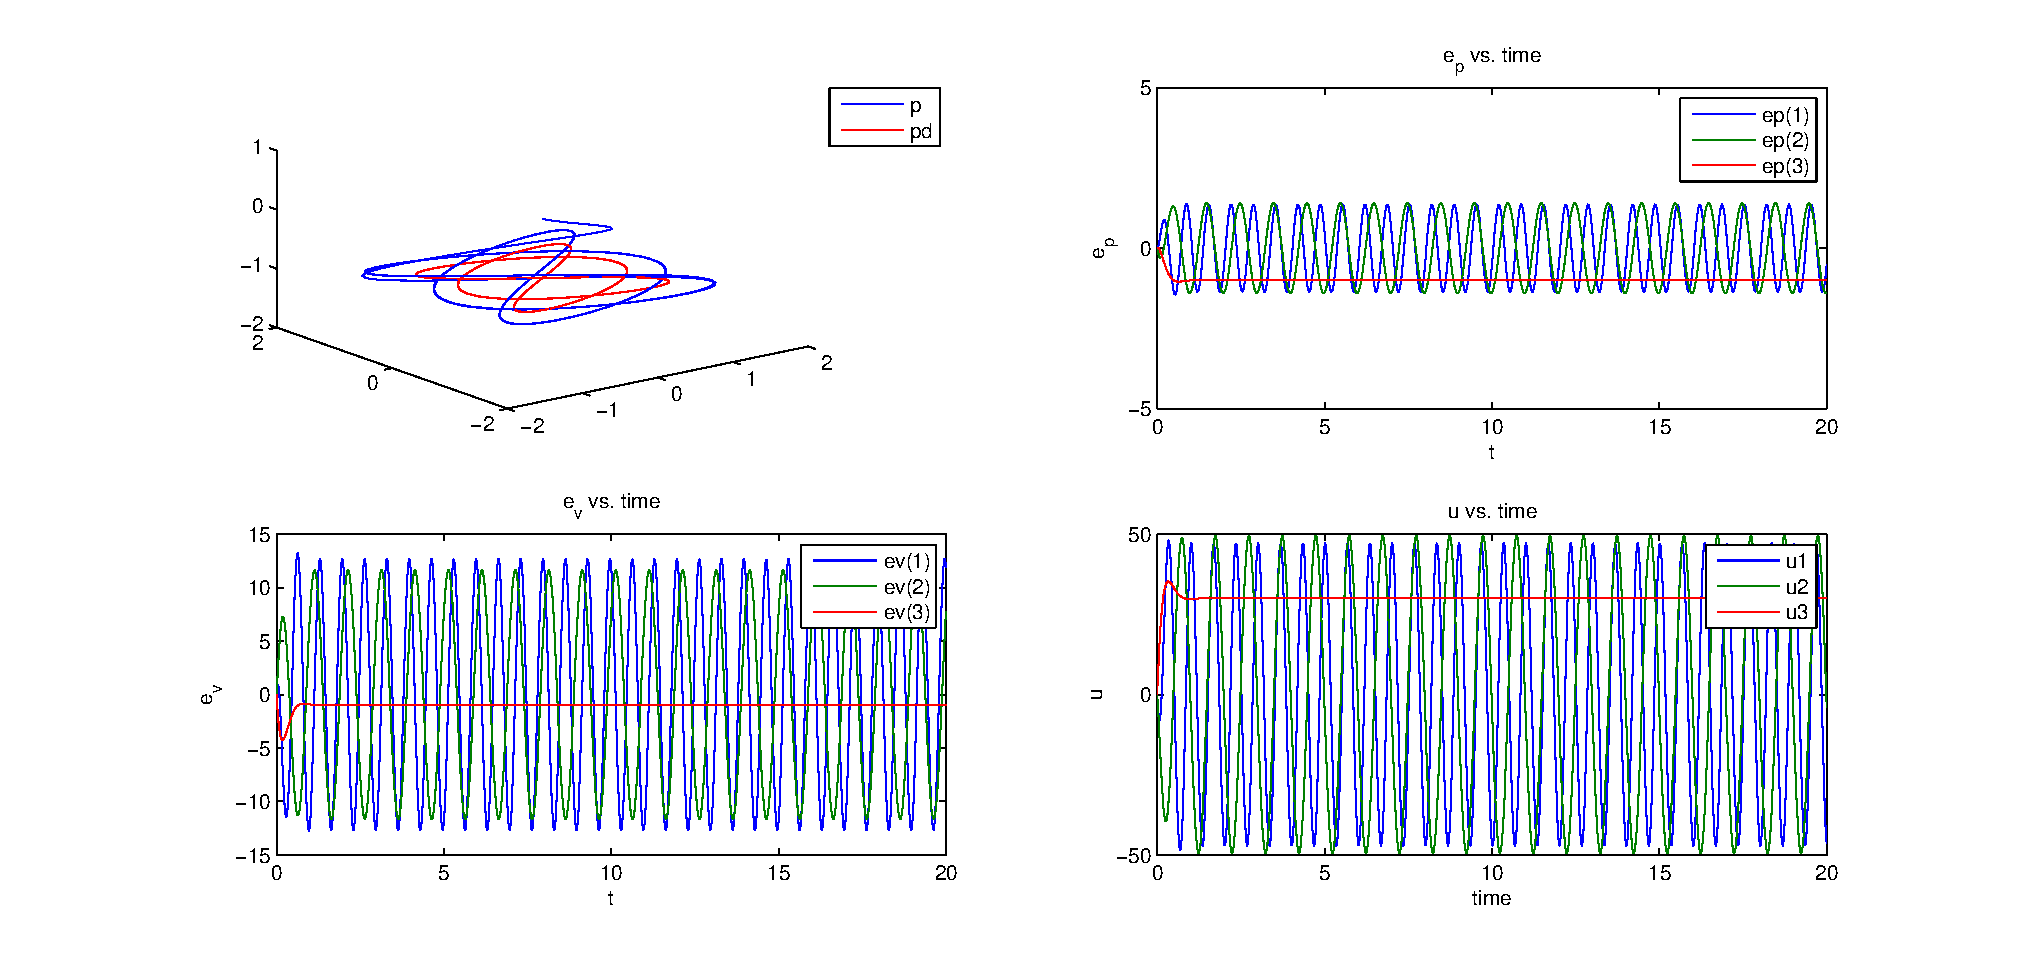
\includegraphics[scale=0.5]{prob5f}
\end{figure} 


\newpage

\section{Problem 6}
a) The equilibrium points at $\dot{x}=0$ are found by:
\begin{align}
\dot{x} &= \begin{bmatrix} \dot{\Omega} \\ \dot{g}\end{bmatrix} \\
&=  \begin{bmatrix}
J^{-1}u-J^{-1}\Omega\times J\Omega \\ -\Omega\times g
\end{bmatrix} \\
&=  \begin{bmatrix}
J^{-1}(-k\Omega + g\times s)-J^{-1}\Omega\times J\Omega \\ -\Omega\times g
\end{bmatrix}
\end{align}
$x_2=0$ only when $\Omega=0$, and then for $x_1=0, g= \pm s$. So the two equilibria are at $x^*=\begin{bmatrix}
0 & s \end{bmatrix}^T, \begin{bmatrix} 0 & -s \end{bmatrix}^T$. \\

b) $V$ can be rewritten as $V=1/2\Omega^TJ\Omega + 1/2(g+s)^T(g+s)$. Since $J$ is positive by definition, $V$ is positive definite. $V=0$ implies we are looking at the second equilibrium, $s^E=\begin{bmatrix} 0 & -s \end{bmatrix}^T$, and if $V$ is p.d. and $\dot{V}$ is n.d., then this implies that $g$ is aligned with $s$.
\begin{align}
\dot{V} &= \dot{\Omega}J+(\dot{g}+s) \\
&=[J^{-1}u-J^{-1}\Omega\times J\Omega]J + [\Omega\times g-s]
\end{align}
The sign indefinite terms are: 
\begin{align}
J^{-1}\Omega\times J\Omega J &= -\Omega J\times J^{-1}\Omega J = 0.
g\times s &= 0
\end{align}
Therefore, $\dot{V}$ is n.d. Breaking $V$ into parts, 
\begin{align}
\frac{1}{2}\gamma_{min}(J) &\leq \frac{1}{2}\Omega^TJ\Omega \\
\frac{1}{2} &\leq \frac{1}{2}(g+s)^T(g+s)
\end{align}
Therefore, the ROA can be estimated as a ball with radius $\frac{1}{2}(min(J)+1)$.


\end{document}